% Sección: Definición del problema
% Definición formal de grid pathfinding con murallas, minas y vidas,
% contextualizada en la navegación del rover Sansano-1.

El terreno de exploración se modela como una cuadrícula $G$ de $N$ filas y $M$ columnas. Cada celda $(i,j)$, con $1 \leq i \leq N$ y $1 \leq j \leq M$, posee un \textbf{identificador de tipo} $t_{i,j} \in \{1, 0, -1\}$ y un \textbf{valor científico} entero $g_{i,j}$ (el cual puede ser positivo, cero o negativo):

\begin{itemize}
  \item \textbf{Celda transitable} ($t_{i,j} = 1$): al transitar por ella, el rover suma $g_{i,j}$ al puntaje acumulado (valores positivos representan muestras geológicas valiosas; valores negativos corresponden a zonas de terreno inestable o radiación).
  \item \textbf{Muralla} ($t_{i,j} = 0$): formaciones rocosas o abismos infranqueables. El rover no puede ingresar a estas celdas bajo ninguna circunstancia.
  \item \textbf{Mina} ($t_{i,j} = -1$): artefacto explosivo enterrado. El rover puede ingresar a la celda, pero al hacerlo detona la mina: el blindaje absorbe el impacto consumiendo \textbf{una vida} y se restan $P$ puntos al puntaje total por concepto de daños en el sistema. Su valor científico $g_{i,j}$ se ignora.
\end{itemize}

El rover \emph{Sansano-1} inicia su trayecto en la celda de aterrizaje $(1,1)$ equipado con $V$ unidades de blindaje (vidas) y tiene como destino la estación de extracción situada en la celda $(N,M)$. Debido a las limitaciones mecánicas de su sistema de tracción y a la pendiente del terreno, desde una celda $(i,j)$ solo se permiten dos maniobras de navegación:
\begin{itemize}
  \item \textbf{Derecha / Este} (\texttt{R}): avanzar a la celda $(i, j+1)$, si $j < M$.
  \item \textbf{Abajo / Sur} (\texttt{D}): avanzar a la celda $(i+1, j)$, si $i < N$.
\end{itemize}

Si en algún momento las vidas del rover llegan a $0$, este queda inoperativo y el camino se considera \textbf{inválido}. Por tanto, una trayectoria es válida si y solo si no atraviesa ninguna muralla y detona a lo más $V-1$ minas a lo largo de su recorrido. Se garantiza que la celda de partida $(1,1)$ y la de llegada $(N,M)$ son siempre celdas normales seguras.

Formalmente, un camino es una secuencia de celdas $C = (c_1, c_2, \dots, c_{N+M-1})$ con $c_1 = (1,1)$, $c_{N+M-1} = (N,M)$ y donde cada celda sucesiva $c_{k+1}$ proviene de $c_k$ mediante un movimiento válido. Denotando por $\mathrm{minas}(C)$ la cantidad de minas detonadas por el camino $C$, el puntaje total obtenido es:
\[
  s(C) = \left( \sum_{\substack{k=1}}^{N+M-1} g_{c_k} \right) \;-\; P \cdot \mathrm{minas}(C),
\]
y el objetivo es encontrar un camino válido $C^{*}$ que maximice dicho puntaje:
\[
  s(C^{*}) = \max_{C \text{ válido}} s(C).
\]
Todo trayecto válido está conformado por exactamente $N-1$ movimientos hacia el sur (\texttt{D}) y $M-1$ movimientos hacia el este (\texttt{R}), totalizando $\binom{N+M-2}{N-1}$ caminos posibles en la cuadrícula.

\begin{mdframed}[linecolor=blue!60!black, backgroundcolor=blue!5,
                 linewidth=1pt, roundcorner=5pt, innertopmargin=8pt,
                 innerbottommargin=8pt]
\textbf{Nota técnica:} Debido a que el rover solo se desplaza hacia el este y hacia el sur, ningún camino puede visitar la misma celda en más de una ocasión; en consecuencia, los valores negativos no inducen ciclos infinitos. Además, sacrificar deliberadamente una unidad de blindaje al detonar una mina puede resultar una estrategia rentable si permite habilitar el paso hacia sectores de alto valor científico.
\end{mdframed}

\subsection{Regla greedy}\label{subsec:regla-greedy}
Para que las soluciones heurísticas sean directamente comparables entre todos los estudiantes, el algoritmo \textsc{greedy} debe implementar con precisión el protocolo de navegación local establecido a continuación:

\begin{mdframed}[linecolor=blue!60!black, backgroundcolor=blue!5,
                 linewidth=1pt, roundcorner=5pt, innertopmargin=8pt,
                 innerbottommargin=8pt]
\textbf{Regla greedy:} Estando en la celda $(i,j)$ con $v$ vidas restantes, los sensores del rover evalúan como \emph{candidatas} las celdas contiguas accesibles (derecha y abajo) que no sean murallas y que no sean minas si $v = 1$ (para evitar la destrucción inminente). La \emph{ganancia neta} de una celda candidata es su valor $g$ si es una celda normal, y $-P$ si es una mina. El rover avanza hacia la candidata de \textbf{mayor ganancia neta}; en caso de empate, prioriza el movimiento hacia la \textbf{derecha}. Si ninguna de las dos celdas vecinas es transitable de forma segura, el algoritmo \textbf{falla} y se declara \texttt{SIN SOLUCION}.
\end{mdframed}

Esta regla no garantiza alcanzar el óptimo global, e incluso puede conducir al rover a callejones sin salida. La \Cref{fig:ejemplo-grilla} ilustra una situación donde la decisión voraz produce una solución subóptima frente a la estrategia global óptima.

% Dibujo de la grilla de ejemplo (N = 4, M = 5).
% Murallas: celdas negras. Minas: celdas marcadas con M.
\newcommand{\minacelda}{\textcolor{red!70!black}{\textbf{M}}}
\newcommand{\grillaejemplo}{%
  \foreach \i/\j in {1/2,3/0} {
    \fill[black!70] (\j,-\i) rectangle ++(1,-1);
  }
  \foreach \fila [count=\i from 0] in {{1,\minacelda,8,8,8},{2,3,{},-2,6},{-3,4,-2,-3,2},{{},-4,1,2,1}} {
    \foreach \valor [count=\j from 0] in \fila {
      \draw (\j,-\i) rectangle ++(1,-1);
      \node at (\j+0.5,-\i-0.5) {\(\valor\)};
    }
  }%
}

\begin{figure}[H]
  \centering
  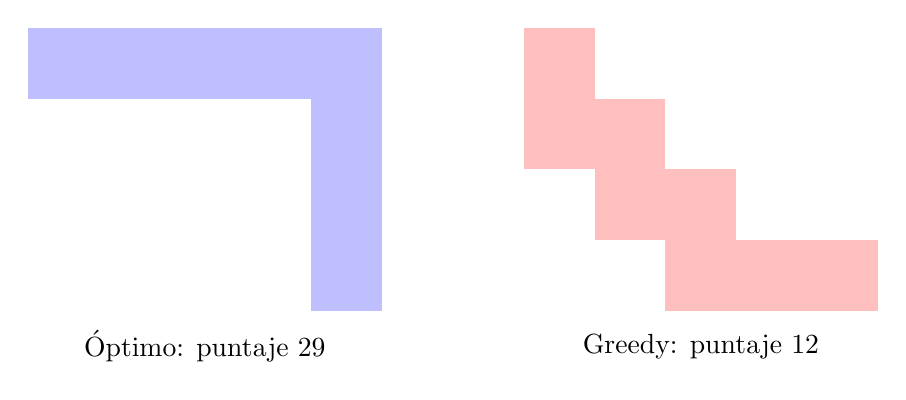
\begin{tikzpicture}[scale=0.9]
    % Camino óptimo (programación dinámica / fuerza bruta)
    \begin{scope}
      \foreach \i/\j in {0/0,0/1,0/2,0/3,0/4,1/4,2/4,3/4} {
        \fill[blue!25] (\j,-\i) rectangle ++(1,-1);
      }
      \grillaejemplo
      \node at (2.5,-4.5) {Óptimo: puntaje $29$};
    \end{scope}
    % Camino greedy
    \begin{scope}[xshift=7cm]
      \foreach \i/\j in {0/0,1/0,1/1,2/1,2/2,3/2,3/3,3/4} {
        \fill[red!25] (\j,-\i) rectangle ++(1,-1);
      }
      \grillaejemplo
      \node at (2.5,-4.5) {Greedy: puntaje $12$};
    \end{scope}
  \end{tikzpicture}
  \caption{Grilla de ejemplo con $N = 4$, $M = 5$, $V = 2$ y $P = 5$. Las murallas se muestran en negro y las minas con la letra M. A la izquierda, el camino óptimo \texttt{RRRRDDD} (puntaje $29$), que asume detonar una mina para acceder al corredor de alto valor superior y concluye con $1$ vida. A la derecha, el camino obtenido por la regla greedy \texttt{DRDRDRR} (puntaje $12$), que evade la mina de forma conservadora. Note que para $V=1$, la solución óptima habría coincidido con la solución encontrada por la estrategia greedy.}
  \label{fig:ejemplo-grilla}
\end{figure}
